% !TEX program = tectonic
% FICHE V2 — écrite à neuf, une page par partie du notebook Portefeuilles_House_Complet
\documentclass[10pt,a4paper,landscape]{article}
\usepackage[margin=0.8cm]{geometry}
\usepackage[T1]{fontenc}
\usepackage[utf8]{inputenc}
\usepackage{lmodern}
\usepackage[french]{babel}
\usepackage{amsmath,amssymb}
\usepackage{booktabs,tabularx}
\usepackage{xcolor}
\usepackage{graphicx}
\usepackage{tikz}
\usetikzlibrary{positioning,arrows.meta}
\definecolor{bleu}{RGB}{20,77,144}
\definecolor{vert}{RGB}{20,110,60}
\definecolor{vertc}{RGB}{90,168,120}
\definecolor{orange}{RGB}{196,123,0}
\definecolor{rouge}{RGB}{160,30,30}
\definecolor{grisf}{RGB}{100,100,100}
\newcommand{\chb}{{\color{bleu}\rule{2.1mm}{2.1mm}}}
\newcommand{\chv}{{\color{vert}\rule{2.1mm}{2.1mm}}}
\newcommand{\cho}{{\color{orange}\rule{2.1mm}{2.1mm}}}
\pagestyle{empty}
\setlength{\parindent}{0pt}
\begin{document}

% ════════════ PAGE 1 — L'IDÉE ET LE DESIGN ════════════
\begin{center}
{\LARGE\bfseries Portefeuilles House, complet --- l'idée, le design, le double verdict}\\[0.6mm]
{\small notebook \texttt{Portefeuilles\_House\_Complet} $\cdot$ House 2014-2026 $\cdot$ 61 cellules exécutées, chaque chiffre sort d'une cellule $\cdot$
couleurs : {\color{bleu}\textbf{PTR}} $\cdot$ {\color{vert}\textbf{photos}} $\cdot$ {\color{orange}\textbf{O/A/T}} $\cdot$ runs {\color{rouge}\textbf{A}}/{\color{vert}\textbf{D}}}
\end{center}
\vspace{1mm}

\begin{center}
\begin{tikzpicture}[x=1cm, y=1cm,
  b/.style 2 args={rectangle, rounded corners=3pt, draw=#1, fill=#1!8, thick,
                   text width=#2, align=center, inner sep=6pt, font=\small}]

\node[b={grisf}{25.8cm}] at (13.4, 15.2)
  {\textbf{128\,960} trades ({\color{bleu}107\,976 PTR} $+$ {\color{orange}20\,984 O/A/T}) \quad$\cdot$\quad
   \textbf{437} membres qui tradent \quad$\cdot$\quad {\color{vert}\textbf{160}} portefeuilles d'entrée injectés \quad$\cdot$\quad
   \textbf{11} années vs SPY (seuil $t_{10} \approx 1{,}81$)};

% frise
\node[font=\small\bfseries, anchor=west] at (0.6, 13.5) {La vie d'une information --- et ce que l'ancienne stratégie en voyait};
\draw[->, thick, grisf] (0.8, 11.7) -- (12.6, 11.7);
\fill[grisf] (1.6, 11.7) circle (0.09);
\node[font=\scriptsize, align=center] at (1.6, 11.2) {transaction $\tau$};
\fill[vert] (2.6, 11.7) circle (0.11);
\node[font=\scriptsize\bfseries, text=vert, align=center] at (3.0, 10.8) {photo Schedule A, au dépôt :\\ tout le patrimoine, une fois};
\fill[bleu] (4.1, 11.7) circle (0.11);
\node[font=\scriptsize\bfseries, text=bleu, align=center] at (4.1, 12.4) {PTR\\ méd. 27 j};
\fill[orange] (10.6, 11.7) circle (0.11);
\node[font=\scriptsize\bfseries, text=orange, align=center] at (10.6, 12.4) {rapport annuel O/A/T\\ méd. 373 j};
\node[b={grisf}{11.6cm}, anchor=north west] at (0.6, 9.9)
  {{\scriptsize l'ancienne stratégie $=$ les {\color{bleu}\textbf{PTR}} seuls, portefeuilles reconstruits \textbf{à partir de zéro} ---
   symptôme : \textbf{937 M\$} de ventes déclarées qu'elle ne peut pas exécuter}};

% matrice 2x2
\node[font=\small\bfseries, anchor=west] at (14.2, 13.5) {Le design : 4 reconstructions, même stratégie, seules les données changent};
\node[b={grisf}{4.6cm}] at (17.6, 11.3) {\textbf{A} --- témoin\\ {\scriptsize\chb\ PTR, départ zéro}\\ \textbf{226} membres};
\node[b={orange}{4.6cm}] at (23.4, 11.3) {\textbf{C}\\ {\scriptsize\chb\cho\ $+$ trades O/A/T}\\ \textbf{380} membres};
\node[b={vert}{4.6cm}] at (17.6, 8.8) {\textbf{B}\\ {\scriptsize\chb\chv\ $+$ photos d'entrée}\\ \textbf{257} membres};
\node[b={bleu}{4.6cm}] at (23.4, 8.8) {\textbf{D} --- adaptée\\ {\scriptsize\chb\chv\cho\ les deux}\\ \textbf{400} membres};
\node[font=\scriptsize, text=orange, anchor=south] at (23.4, 12.5) {$+$ O/A/T $\rightarrow$};
\node[font=\scriptsize, text=vert, rotate=90, anchor=south] at (15.9, 8.8) {$+$ photo $\rightarrow$};

\node[b={grisf}{25.8cm}] at (13.4, 6.6)
  {\textbf{l'identification} :\quad B $-$ A $=$ \textbf{\color{vert}effet photo}\qquad C $-$ A $=$ \textbf{\color{orange}effet O/A/T}\qquad
   D $-$ B $-$ C $+$ A $=$ \textbf{interaction}\\[0.4mm]
   {\scriptsize même stratégie partout : classement Sharpe (éligible $n_j \ge 126$ et Sharpe $> 0{,}4$) $\cdot$ $K^*$ walk-forward $\cdot$ poids $1/K$ $\cdot$ tenue 1 an}};

\node[b={rouge}{25.8cm}] at (13.4, 4.5)
  {\textbf{le double verdict} :\quad \textbf{(1)} la stratégie ne bat toujours pas le SPY ($\max t = 0{,}85$) et les trades O/A/T pèsent négativement ($-2{,}2\,\%$/an apparié)\\
   \textbf{(2)} MAIS la reconstruction adaptée est presque \textbf{10$\times$ plus complète} : rappel des positions déclarées \textbf{6\,\% $\to$ 57\,\%}, à précision égale (p.\,5)};

\node[font=\scriptsize, text=grisf] at (13.4, 3.1)
  {p.\,2 les membres : qui a quoi $\cdot$ p.\,3 les transactions : les livres de comptes $\cdot$ p.\,4 la reconstruction $\cdot$
   \textbf{p.\,5 la vérification} $\cdot$ p.\,6 la stratégie $\cdot$ p.\,7 conclusion};

\end{tikzpicture}
\end{center}

\newpage
% ════════════ PAGE 2 — P1 · LES MEMBRES ════════════
\begin{center}
{\Large\bfseries 2 $\cdot$ P1 --- Les membres : qui est qui, qui a quoi}\\[0.5mm]
{\scriptsize en 10 secondes : sur 900 membres, 437 tradent --- et l'information disponible varie énormément d'un membre à l'autre}
\end{center}

\begin{center}
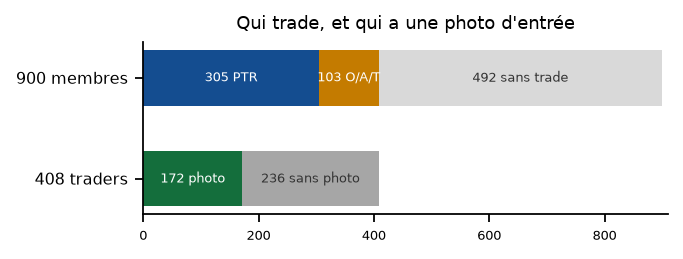
\includegraphics[width=0.66\textwidth]{figures/fig_10_partition.png}
\end{center}

\noindent\begin{minipage}[t]{0.40\textwidth}\vspace{0pt}
\textbf{La typologie} {\scriptsize(partition exhaustive des 900, depuis la matrice d'information membre $\times$ source)}
\begin{center}\small
\begin{tabular}{@{}lr@{}}
\toprule
équipés \textbf{complets} (photo $+$ trades $+$ O $+$ T) & \textbf{49} \\
photo $+$ trades $+$ O (pas encore de T) & 113 \\
trades $+$ photo OU O (partiels) & 257 \\
trades seulement & 18 \\
aucun trade exploitable & 463 \\
\midrule
total registre & 900 \\
\bottomrule
\end{tabular}
\end{center}
\begin{itemize}
\item[--] les identités bouclent, par assert : $900 = 305 + 132 + 463$ et $437 = 166 + 271$ ;
\item[--] \textbf{132 membres} n'existent QUE dans les rapports annuels --- 30\,\% des traders, invisibles pour l'ancienne stratégie ;
\item[--] \textbf{459 membres} ont $\geq 1$ photo annuelle O exploitable (2\,173 documents) : l'assiette du juge de la p.\,5.
\end{itemize}
\end{minipage}\hfill
\begin{minipage}[t]{0.57\textwidth}\vspace{0pt}
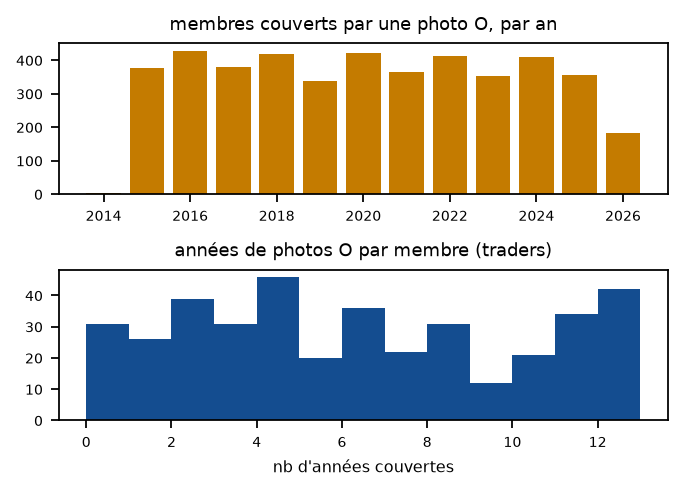
\includegraphics[width=\linewidth]{figures/fig_10_couverture_O.png}\\[0.5mm]
{\scriptsize la couverture des rapports annuels O : $\sim$350-430 membres couverts chaque année --- le patrimoine du Congrès est observable en continu, pas seulement à l'entrée.}
\end{minipage}

\newpage
% ════════════ PAGE 3 — P2 · LES TRANSACTIONS ════════════
\begin{center}
{\Large\bfseries 3 $\cdot$ P2 --- Les transactions : les livres de comptes, marche par marche}\\[0.5mm]
{\scriptsize chaque marche est une cellule avec assert d'identité (total $-$ marches $=$ retenu) --- rien n'est écarté sans raison affichée}
\end{center}

\noindent\begin{minipage}[t]{0.32\textwidth}\vspace{0pt}
{\color{orange}\rule{3mm}{3mm}}\ \textbf{\color{orange}Trades O/A/T : 26\,115 $\to$ 20\,984}
\begin{center}\scriptsize
\begin{tabular}{@{}lr@{}}
\toprule
lignes table 16 (sans écho PTR) & 26\,115 \\
$-$ exchanges (sens E) & $-221$ \\
$-$ dates hors 2013-2026 & $-14$ \\
$-$ sans montant & $-0$ \\
$-$ ticker corrompu (garde-fou) & $-48$ \\
$-$ aucune série de prix$^{\dagger}$ & $-4\,367$ \\
$-$ collision exacte avec nos PTR$^{\ddagger}$ & $-481$ \\
\midrule
\textbf{= retenus (provenance oat)} & \textbf{20\,984} \\
\bottomrule
\end{tabular}
\end{center}
{\scriptsize $^{\dagger}$ après tentative de téléchargement --- EIF puis les fonds monétaires (SPAXX, FZDXX\ldots). $^{\ddagger}$ 490 appariements : 9 lignes matchent 2 lots PTR du même jour. $\approx$ 16\,\% du flux total.}
\end{minipage}\hfill
\begin{minipage}[t]{0.32\textwidth}\vspace{0pt}
{\color{bleu}\rule{3mm}{3mm}}\ \textbf{\color{bleu}Membres : 370 $\to$ 437 qui tradent}
\begin{center}\scriptsize
\begin{tabular}{@{}lr@{}}
\toprule
membres dans la table 16 brute & 370 \\
$-$ aucune ligne O/A/T exploitable & $-33$ \\
\quad {\color{grisf}dont repêchés par leurs PTR} & {\color{grisf}15} \\
\quad {\color{grisf}dont vraiment sortis} & {\color{grisf}18} \\
\midrule
= membres O/A/T exploitables & 337 \\
\quad dont : ont aussi des PTR & 205 \\
\quad dont : \textbf{O/A/T seulement} & \textbf{132} \\
$\cup$ membres PTR (non-régression : identique) & 305 \\
\midrule
\textbf{= population qui trade} & \textbf{437} \\
\bottomrule
\end{tabular}
\end{center}
{\scriptsize PTR inchangés au trade près : $107\,976$ / $305$ (asserté).}
\end{minipage}\hfill
\begin{minipage}[t]{0.32\textwidth}\vspace{0pt}
{\color{vert}\rule{3mm}{3mm}}\ \textbf{\color{vert}Photos : 284 $\to$ 160 injectées}
\begin{center}\scriptsize
\begin{tabular}{@{}lr@{}}
\toprule
photos déposées (252 H $+$ 32 C) & 284 \\
$-$ aucune ligne tickérisée et valorisée & $-36$ \\
\midrule
= photos exploitables & 248 \\
$-$ aucun prix au 1\ier{} jour coté $\geq$ dépôt & $-20$ \\
\midrule
= membres initialisables ($h_0$) & 228 \\
\quad dont : tradent $\to$ \textbf{injectés} & \textbf{160} \\
\quad dont : aucun trade & 68 \\
\bottomrule
\end{tabular}
\end{center}
{\scriptsize 75,3\,\% de la valeur convertie en parts $\cdot$ médiane 387\,505 \$, max 78,3 M\$ $\cdot$ B injecte 117 (PTR), D les 160.}
\end{minipage}

\vspace{2mm}
\noindent\begin{minipage}[t]{0.51\textwidth}\vspace{0pt}
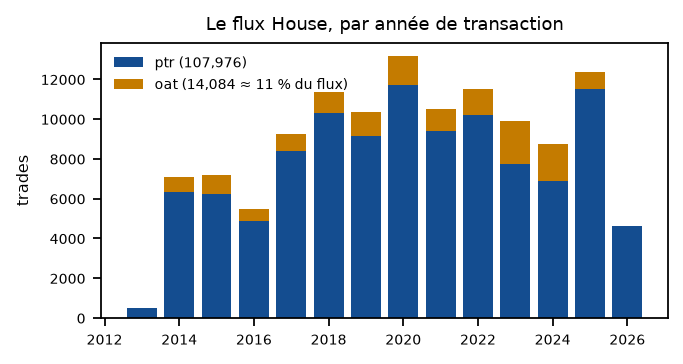
\includegraphics[width=\linewidth]{figures/fig_10_flux.png}
\end{minipage}\hfill
\begin{minipage}[t]{0.46\textwidth}\vspace{0pt}
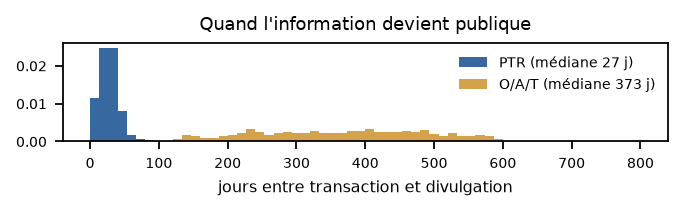
\includegraphics[width=\linewidth]{figures/fig_10_delais.png}\\[0.3mm]
{\scriptsize délais recalculés : \textbf{PTR 27 j} (q90 49) vs \textbf{O/A/T 373 j} (q90 540) --- le PTR est un signal, l'annuel un enregistrement.}
\end{minipage}

\newpage
% ════════════ PAGE 4 — P3 · LA RECONSTRUCTION ════════════
\begin{center}
{\Large\bfseries 4 $\cdot$ P3 --- La reconstruction : le portefeuille de chaque membre}\\[0.5mm]
{\scriptsize en 10 secondes : la photo change le point de départ, rend les ventes exécutables --- et le classement change à toutes les coupes}
\end{center}

\noindent\begin{minipage}[t]{0.44\textwidth}\vspace{0pt}
\textbf{Les maths, en trois lignes} {\scriptsize($m$ = membre, $i$ = ticker, $h$ = parts, $\tilde v$ = milieu de fourchette)}
$$h_0(m,i) = \tilde v_i / P_i(\tau(f_0)) \quad \text{au jour du \textbf{dépôt} de la photo}$$
$$\text{achat : } h \mathrel{+}= \tilde v / P(\tau(t)) \qquad \text{vente : } h \mathrel{-}= \min(q, h)$$
$$r_m(t) = \frac{\sum_i h_i(t{-}1)\, P_i(t)}{\sum_i h_i(t{-}1)\, P_i(t{-}1)} - 1 \quad \text{(parts de la \textbf{veille})}$$
{\scriptsize un apport (photo ou achat) n'est jamais une performance --- $r = 0$ exactement au jour d'injection, testé.}

\vspace{1.5mm}
\textbf{Les 4 reconstructions}
\begin{center}\small
\begin{tabular}{@{}lrrr@{}}
\toprule
run & membres & photos inj. & ventes tronquées \\
\midrule
\chb\ A témoin & 226 & 0 & 937 M\$ \\
\chb\chv\ B & 257 & 117 & 897 M\$ \\
\chb\cho\ C & 380 & 0 & 1\,337 M\$ \\
\chb\chv\cho\ \textbf{D adaptée} & \textbf{400} & \textbf{160} & 1\,278 M\$ \\
\bottomrule
\end{tabular}
\end{center}
\begin{itemize}
\item[--] pourquoi A $= 226 < 305$ : \textbf{77 vendeurs purs} (que des ventes) n'ont jamais de portefeuille en partant de zéro --- la photo en \textbf{ressuscite 31} dans B ;
\item[--] à la coupe 2021 : \textbf{152} éligibles dans A, \textbf{241} dans D ($+95$ entrants, $-6$ sortants --- scatter ci-contre) ;
\item[--] la sélection du top-$K$ diffère entre A et D à \textbf{11 coupes sur 11}.
\end{itemize}
{\scriptsize\color{grisf}preuves du moteur : recalcul naïf en double boucle $=$ 869 rendements identiques $\cdot$ B $\equiv$ A hors photos $\cdot$ bloc 2018 de la stratégie recalculé à la main $\equiv$ moteur.}
\end{minipage}\hfill
\begin{minipage}[t]{0.53\textwidth}\vspace{0pt}
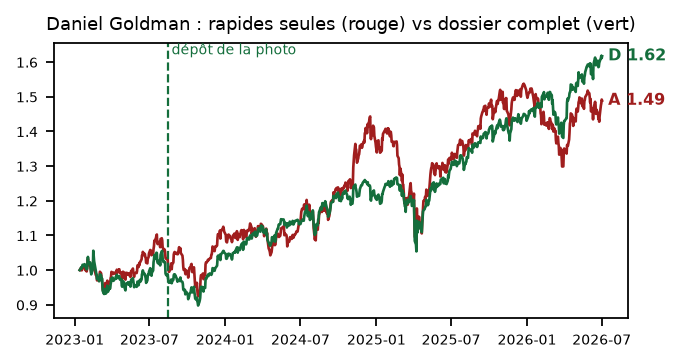
\includegraphics[width=\linewidth]{figures/fig_10_filrouge.png}\\[1mm]
\begin{center}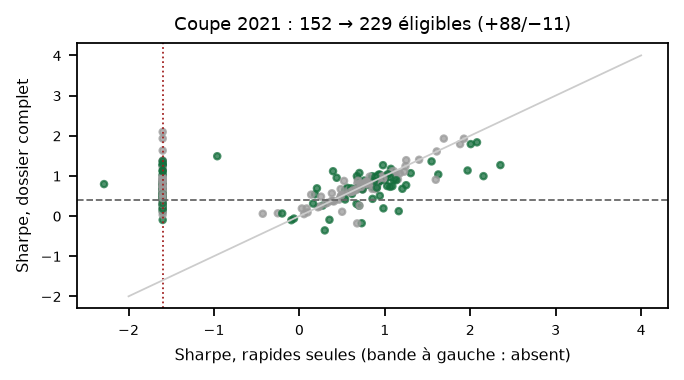
\includegraphics[width=0.76\linewidth]{figures/fig_10_sharpe_shift.png}\end{center}
\end{minipage}

\newpage
% ════════════ PAGE 5 — P4 · LA VÉRIFICATION ════════════
\begin{center}
{\Large\bfseries 5 $\cdot$ P4 --- La vérification : les rapports annuels jugent la reconstruction}\\[0.5mm]
{\scriptsize en 10 secondes : le témoin ne retrouve que 6\,\% des positions que les élus déclarent chaque année --- la reconstruction adaptée en retrouve 57\,\%, à précision égale}
\end{center}

\noindent\begin{minipage}[t]{0.42\textwidth}\vspace{0pt}
\textbf{La méthode.} Chaque photo O déclare le patrimoine au 31/12. À la date de \textbf{dépôt} de l'O, on confronte reconstruction et déclaration :
\begin{itemize}
\item[--] \textbf{(a) positions} : précision $=$ part du reconstruit qui est déclaré $\cdot$ rappel $=$ part du déclaré qu'on a reconstruit ;
\item[--] \textbf{(b) valeurs} : sur les positions communes, $h \cdot P \in [\underline v, \bar v]$ ?
\end{itemize}
Assiette : \textbf{2\,173 photos O} $\cdot$ 459 membres $\cdot$ 3\,242 confrontations (A et D).

\vspace{1.5mm}
\textbf{Le verdict}
\begin{center}\small
\begin{tabular}{@{}lccc@{}}
\toprule
 & A témoin & D adaptée & \\
\midrule
rappel médian & 6\,\% & \textbf{57\,\%} & $\nearrow\nearrow$ \\
précision médiane & 60\,\% & 59\,\% & $\approx$ \\
valeurs en fourchette & 53\,\% & 52\,\% & $\approx$ \\
\bottomrule
\end{tabular}
\end{center}
\begin{itemize}
\item[--] le \textbf{T} en réconciliation finale : 122 photos de sortie, rappel 63\,\%, précision 60\,\% ;
\item[--] validation : une photo recomptée à la main $\equiv$ la table (assert) ;
\item[--] limites : clés ticker seulement $\cdot$ fourchettes larges $\cdot$ photo au 31/12 confrontée au jour du dépôt (bruit symétrique A/D) $\cdot$ amendements non re-fusionnés.
\end{itemize}
\textbf{La lecture} : les corrections rendent le portefeuille reconstruit presque \textbf{10$\times$ plus complet}
sans dégrader la justesse --- la preuve, indépendante de toute performance boursière, que l'exploitation
des filing types améliore la donnée.
\end{minipage}\hfill
\begin{minipage}[t]{0.55\textwidth}\vspace{0pt}
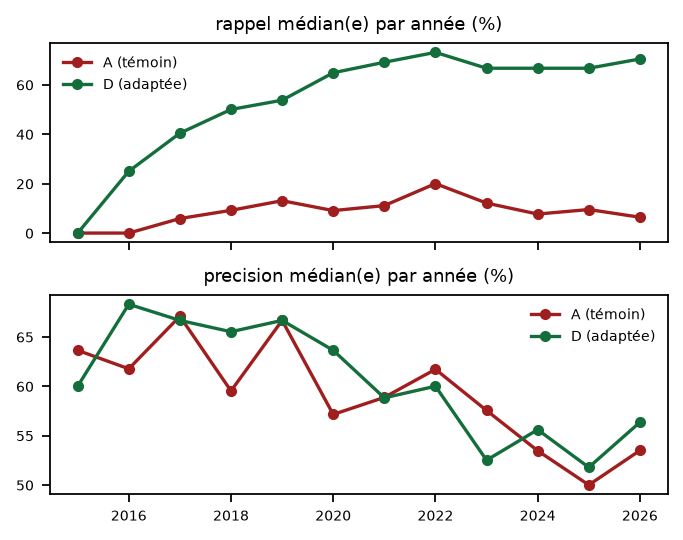
\includegraphics[width=\linewidth]{figures/fig_10_verif_O.png}\\[0.5mm]
{\scriptsize rappel (gauche) et précision (droite) médians par année : l'écart de rappel est massif et stable --- le témoin, qui part de zéro et ne voit que les PTR, passe à côté de l'essentiel du patrimoine déclaré.}
\end{minipage}

\newpage
% ════════════ PAGE 6 — P5 · LA STRATÉGIE ════════════
\begin{center}
{\Large\bfseries 6 $\cdot$ P5 --- La stratégie : le verdict change-t-il ?}\\[0.5mm]
{\scriptsize en 10 secondes : aucun $t$ au-dessus du seuil, l'effet O/A/T est négatif, et le $+6{,}6\,\%$ de B vient d'une seule année}
\end{center}

\noindent\begin{minipage}[t]{0.46\textwidth}\vspace{0pt}
\textbf{Le tableau central} {\scriptsize(poids $1/K$ ; 11 années ; seuil $t_{10} \approx 1{,}81$)}
\begin{center}\small
\begin{tabular}{@{}lrrlrrr@{}}
\toprule
run & excès/an & $t$ & gagn. & $\beta$ & $\alpha$/an & $t_{\text{ap}}$ \\
\midrule
\chb\ A témoin & $+0{,}9\,\%$ & $0{,}37$ & 4/11 & $0{,}99$ & $+0{,}6$ & $0{,}28$ \\
\chb\chv\ \textbf{B} & $\mathbf{+6{,}6\,\%}$ & $\mathbf{0{,}85}$ & 5/11 & $0{,}98$ & $+5{,}2$ & $\mathbf{1{,}55}$ \\
\chb\cho\ C & $-1{,}3\,\%$ & $-0{,}77$ & 3/11 & $0{,}83$ & $+1{,}0$ & $0{,}65$ \\
\chb\chv\cho\ \textbf{D adaptée} & $-1{,}6\,\%$ & $-0{,}61$ & 6/11 & $0{,}85$ & $+0{,}6$ & $0{,}37$ \\
\bottomrule
\end{tabular}
\end{center}
{\scriptsize note : l'inverse-vol, joué partout, fait moins bien que $1/K$ sur les 4 runs ; $1/K$ reste le défaut.}

\vspace{1.5mm}
\textbf{Les effets, en différences appariées} {\scriptsize(mêmes années, même SPY --- test plus puissant que les $t$ marginaux)}
\begin{center}\small
\begin{tabular}{@{}lrr@{}}
\toprule
effet & moyenne (\%/an) & $t$ apparié \\
\midrule
photo (B$-$A) & $+5{,}7$ & $0{,}74$ \\
O/A/T (C$-$A) & $-2{,}2$ & $-0{,}74$ \\
interaction (D$-$B$-$C$+$A) & $-6{,}0$ & $-0{,}89$ \\
\bottomrule
\end{tabular}
\end{center}
\begin{itemize}
\item[--] l'essentiel du $+6{,}6\,\%$ de B vient d'\textbf{une seule année} : 2020, excès $+82{,}5\,\%$ (barres ci-contre) --- d'où le $t$ faible ;
\item[--] \textbf{S2} (stratifié, $1/K$) : aucun $t$ significatif --- A$\cdot$photo $0{,}12$ $\cdot$ A$\cdot$zéro $-0{,}46$ $\cdot$ D$\cdot$photo $-0{,}70$ $\cdot$ D$\cdot$zéro $-0{,}37$ : le signal ne survit pas à la stratification ;
\item[--] \textbf{puissance} : $\hat\sigma = 8{,}5\,\%$/an $\Rightarrow$ MDE $\approx$ \textbf{6,9\,\%/an} --- sous ce niveau, un vrai excès resterait invisible : le nul borne, il ne prouve pas ;
\item[--] $K^*$ walk-forward : B verrouille $4$ ; C et D montent (8-18, puis $\sim$11).
\end{itemize}
\end{minipage}\hfill
\begin{minipage}[t]{0.51\textwidth}\vspace{0pt}
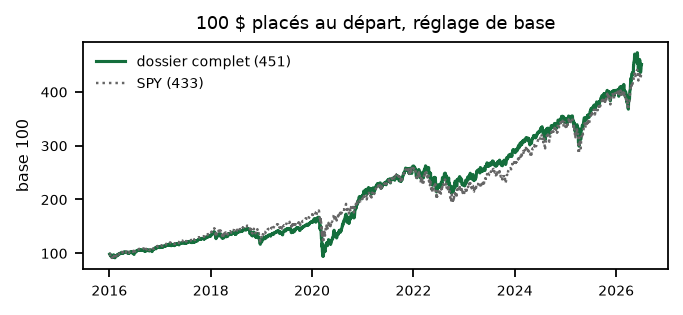
\includegraphics[width=\linewidth]{figures/fig_10_nav.png}\\[1mm]
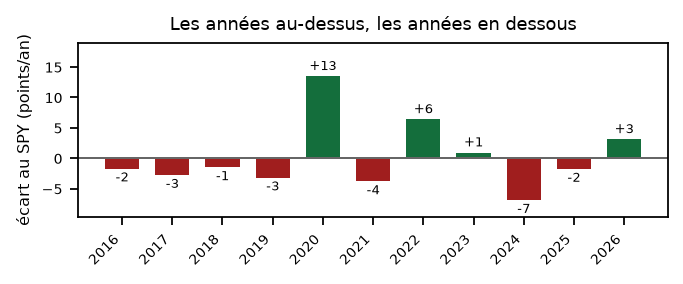
\includegraphics[width=\linewidth]{figures/fig_10_exces_annuel.png}
\end{minipage}

\newpage
% ════════════ PAGE 7 — P6 · CONCLUSION ════════════
\begin{center}
{\Large\bfseries 7 $\cdot$ P6 --- Que conclure, et pourquoi y croire ?}
\end{center}

\noindent\begin{minipage}[t]{0.47\textwidth}\vspace{0pt}
\textbf{\color{rouge}Le double verdict}
\begin{itemize}
\item[--] \textbf{(1)} \textbf{pas d'alpha démontrable} : $\max t = 0{,}85$, effets appariés nuls, $t$ appariés stratifiés $\le 0{,}59$ --- robuste au poids, à la strate, au périmètre ;
\item[--] \textbf{(2)} \textbf{la donnée, elle, est transformée} : reconstruction $10\times$ plus complète (rappel 6\,\% $\to$ 57\,\%), 437 traders au lieu de 305, ventes exécutables ;
\item[--] le seul effet positif (photo, $+6{,}6\,\%$) est concentré sur 2020 et disparaît en stratifiant --- \textbf{mesure plutôt que talent}.
\end{itemize}

\vspace{1.5mm}
\textbf{A $\to$ D, ce qui change}
\begin{center}\small
\begin{tabular}{@{}lccc@{}}
\toprule
 & A témoin & D adaptée & \\
\midrule
membres couverts & 226 & \textbf{400} & $\nearrow$ \\
photos injectées & 0 & \textbf{160} & $\nearrow$ \\
rappel vs photos annuelles & 6\,\% & \textbf{57\,\%} & $\nearrow\nearrow$ \\
$\beta$ & 0,99 & \textbf{0,85} & $\searrow$ \\
$t_{\alpha}$ ajusté & $+0{,}28$ & $+0{,}37$ & $\approx$ \\
excès/an & $+0{,}9\,\%$ & $-1{,}6\,\%$ & $\searrow$ \\
\bottomrule
\end{tabular}
\end{center}

\vspace{1.5mm}
{\footnotesize\textbf{\color{grisf}Pourquoi y croire} : sha256 des tables $\equiv$ manifeste $\cdot$ cascades vérifiées par assert $\cdot$
recalcul naïf 869 rendements identiques $\cdot$ $r = 0$ au jour d'injection $\cdot$ B $\equiv$ A hors photos $\cdot$
bloc 2018 refait à la main $\cdot$ une photo O recomptée à la main $\cdot$ \texttt{prices\_v2} intact $\cdot$ zéro chiffre en dur.}
\end{minipage}\hfill
\begin{minipage}[t]{0.50\textwidth}\vspace{0pt}
\textbf{Limites --- et le test qui trancherait chacune}
\begin{center}\small
\begin{tabularx}{\linewidth}{@{}XXX@{}}
\toprule
limite & conséquence & test qui trancherait \\
\midrule
O/A/T datés à la transaction, divulgués $\sim$373 j après & C et D optimistes par construction (pas jouables tels quels) & re-dater les O/A/T au jour du dépôt --- devrait tuer C \\
double comptage possible (achat PTR pré-dépôt $\subset$ photo) & $h_0$ surestimé pour certains & re-jouer B sans les PTR antérieurs au dépôt \\
24,7\,\% de la valeur des photos non convertie (non-coté) & G\_photo partiellement observé & --- (limite de données) \\
coûts de transaction non modélisés & tout excès net serait plus bas & grille de coûts (5-20 bps) \\
$n = 11$ années & puissance limitée (MDE 6,9\,\%/an) & attendre, ou coupes semestrielles \\
\bottomrule
\end{tabularx}
\end{center}

\vspace{1.5mm}
\textbf{La valeur du travail, même sous le null} : un pipeline de données réparé et \textbf{vérifié contre
2\,173 photos annuelles} --- l'actif sert tel quel à toute stratégie future (ticker, notebook 11).
\end{minipage}

\end{document}
